\section{Interaktion med sociale robotter}
\label{InteraktionSocialeRobotter}
%
Inden der dykkes ned i hvilke parametre, der har indflydelse på hvordan interaktionen med sociale robotter perciperes og accepteres, vil nogle mere generelle tendenser blive diskuteret. Det dækker blandt andet over køns-, alders- samt kulturelleforskelle i henhold til synet på sociale robotter. Dernæst gives der nogle eksempler på, hvordan relaterede studier har målt brugerens perception og accept af sociale robotter.
%
\subsection{Generelle tendenser}
\label{InteraktionSocialeRobotterGenerelleTendenser}
%
I den vestlige verden er vi i langt mindre grad villige til at acceptere sociale robotter end hvad der eksempelvis er tilfældet i Japan, \parencite[s. 28]{PDF:InTheCompanyofRobots}. Det skyldes, ifølge \textcite[s. 28]{PDF:InTheCompanyofRobots}, at der er en indgroede frygt for maskiner og følelsen af manglende kontrol, hvilket ikke er tilfældet i den Japanske kultur, som åndeliggøre robotter. At mennesker i den vestlige verden frygter robotter kan, blandt andet, retfærdiggøres med at i 2012 angav 87 \% af borgerne i Europa at de aldrig har været i kontakt med en robot, hverken i hjemmet eller på ens arbejdsplads, \parencite[s. 40]{PDF:PerceptionAcceptance}. I en undersøgelse, beskrevet af \textcite[s. 41]{PDF:PerceptionAcceptance}, fremgår det at synet på robotter ikke har ændret sig de sidste 35 år. Når robotterne, ved brug af tegninger, visualiseres så minder de i høj grad om robottypen: \textit{Non assistive robots}, illustreret på \autoref{fig:CategorizationOfRobots}. Endvidere tyder det på, at Europærer frygter, at de vil miste deres job til robotten og at robotten er til for at erstatte mennesket, \parencite[s. 22]{PDF:RobotShiftFromIPtoSR}.   

Derudover er der en tendens til, at mænd i højere grad perciperer robotten som menneskeagtig sammenlignet med kvinder, som i langt højere grad perciperer robotten som en maskine, \parencite[s. 28]{PDF:InTheCompanyofRobots}. Ifølge \textcite[s. 1479]{PDF:ExploringInfluencingVariable}, perciperer mænd robotter som værende mere brugbare, de har større intention om at bruge dem og de er mere villige til at acceptere robotter end kvinder er.  

Ydermere argumenterer \textcite[s. 2]{PDF:SharingALifeHarvey} for, at den ældre population i højere grad accepterer sociale robotter, sammenlignet med den yngre population. Det antages, at en af årsagerne til det formentlig skyldes, at der anvendes sociale robotter i ældreplejen eksempelvis til mindske følelsen af ensomhed, \fullref{EksisterendeSocialeRobotter}. I mere praktiske situation, som eksempelvis rengøring, tøjvask og lignende, foretrækker ældre robotter fremfor mennesker, hvorimod hvis opgaverne er omsorgsrelateret foretrækkes mennesker, \parencite[s. 22]{PDF:RobotShiftFromIPtoSR}.

\subsection{Parametre, der har indflydelse på accept og interaktion med sociale robotter}
\label{InteraktionSocialeRobotterParametre}
%
Der er to overordene kategorier af parametre: \textit{Utilitarian} og \textit{Hedonic}, først nævnte dækker over det praktiske og anvendelige aspekt ved at interagere med en social robot, hvor sidst nævnte relateres til brugerens oplevelse af at anvende den sociale robot, \parencite[s. 1476]{PDF:SharingALifeHarvey}. Da disse parametre har indflydelse på hvorvidt brugeren udfører en bestem adfærd, skal der tages højde for følgende:\blankline
%
\begin{quotation}
\textit{
  \begin{enumerate}
  \item the likely positive or negative consequences of the behavior
  \item the approval or disapproval of the behavior by respected individuals or groups, and
  \item the factors that may facilitate or impede performance of the behavior.
\end{enumerate}}
\textcite[s. 1477]{PDF:SharingALifeHarvey}\blankline
\end{quotation}
\noindent
%
Anvendes de tre overvejelser til at undersøge brugerens accept afspejler de, ifølge \textcite[s. 1477]{PDF:SharingALifeHarvey}, henholdvist brugerens evaluering af robotten, hvilke sociale normative overbevisninger der tilskrives robotten ved brug samt hvilke kontekstuelle faktorer der spiller ind ved brug.

\subsubsection*{Utilitarian}
\label{InteraktionSocialeRobotterParametreUtilitarian}
%
Som nævnt dækker \textit{utilitarian} parametre over det praktiske og anvendelige aspekt ved at interagere med en social robot. Derudover har disse parametre ligeledes indflydelse på den specifikke adfærd. I følgende afsnit belyses hvilke parametre der har indflydelse på det praktiske såvel som det anvendelige aspekt. Der tages primært udgangspunkt i \textcite[s. 1477]{PDF:SharingALifeHarvey}.
%
\begin{figure}[H]
\centering
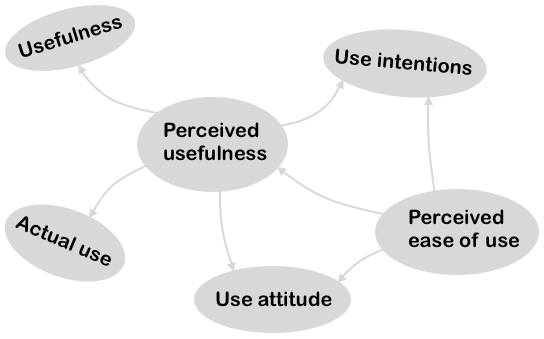
\includegraphics[width = 0.75\textwidth]{Figure/UtilitarianParameters} 
\caption{Sammenhængen mellem de seks forskellige parametre, der har indflydelse på det praktiske og anvendelige aspekt. Pilene indikerer hvilken retning indflydelsen er mellem to parametre.}
\label{fig:UtilitarianParameters}
\end{figure}
\noindent 
%
Baseret på \textcite[s. 1477]{PDF:SharingALifeHarvey} defineres \textit{usefulness} som værende brugerens overbevisning om, at robotten vil forbedre de daglige aktiviteter. Ifølge \textcite[s. 11]{PDF:SharingALifeHarvey} tyder det på, at \textit{usefulness} er en vigtig parametre, der kan bidrage til langtidssigtet forhold mellem bruger og robot. \textit{Ease of use} defineres som værende brugerens overbevisning om, at det nemt at anvende robotten. Derudover argumenterer \textcite[s. 1477]{PDF:SharingALifeHarvey} for, at i situationer hvor robotten skal indgå i en social interaktion med mennesker, er det nødvendigt at robotten gengiver menneskeagtige træk for, at brugeren føler sig komfortabel nok til at indgå i interaktionen. Robottens evne til at tilpasse sig den sociale kontekst afhængigt af brugeres behov, defineres som \textit{perceived adaptability}. Ifølge \textcite[s. 1477]{PDF:SharingALifeHarvey}, har \textit{perceived adaptability} indflydelse på \textit{perceived usefulness}, \textit{use attitude}, \textit{use intentions}, som er repræsenteret på \autoref{fig:UtilitarianParameters}. Derudover har \textit{perceived adaptability} indflydelse på \textit{enjoyment}. Ydermere tyder det på at \textit{intelligence}, har en effekt på hvor realistiske robotten perciperes, \parencite[s. 1477]{PDF:ExploringInfluencingVariable}.   
%
\subsubsection*{Hedonic}
\label{InteraktionSocialeRobotterParametreHedonic}
%
Som nævnt dækker \textit{hedonic} parametre over brugerens oplevelse af at anvende den sociale robot. Derudover har disse parametre ligeledes indflydelse på den specifikke adfærd. I følgende afsnit belyses hvilke parametre der har indflydelse på det dette. Der tages primært udgangspunkt i \textcite[ss. 1477-1478]{PDF:SharingALifeHarvey}. På \autoref{fig:HedonicParameters} illustreres forskellige parametre, samt deres indbyrdes forhold.
%
\begin{figure}[H]
\centering
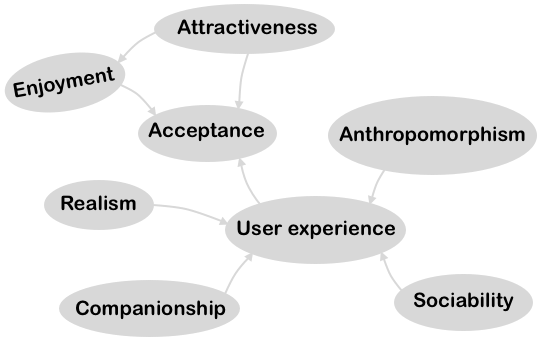
\includegraphics[width = 0.75\textwidth]{Figure/HedonicParameters} 
\caption{Sammenhængen mellem de otte forskellige parametre, der har indflydelse på brugerens oplevelse. Pilene indikerer hvilken retning indflydelsen er mellem to parametre.}
\label{fig:HedonicParameters}
\end{figure}
\noindent 
%
Baseret på \textcite[s. 1477]{PDF:ExploringInfluencingVariable} har både \textit{enjoyment}, der defineres som værende følelsen af fornøjelse eller glæde forbundet med brug, og \textit{attractiveness}, der defineres som værende den positive evaluering af robottens udseende, på flere af de parametre gengivet på \autoref{fig:UtilitarianParameters}. \textit{Enjoyment} har indflydelse på \textit{ease of use}, \textit{use attitude} samt \textit{use intentions}. Derimod har \textit{attractiveness} indflydelse på \textit{usefulness} og \textit{ease of use}. \blankline 
%
Antropomorfisering defineres som værende evnen til at tilskrive naturfænomener, guder, overnaturlige væsner og dyr menneskelige egenskaber, såsom følelser og motiver, \parencite{WEB:DefAntropomorisering}. Dog defineres antropomorfisering i HRI sammenhæng, som værende evnen til at tildele og beskrive objekter med menneskelige egenskaber, for at rationalisere objektets adfærd, \parencite[s. 1478]{PDF:ExploringInfluencingVariable}. Ifølge \textcite[s. 1478]{PDF:ExploringInfluencingVariable} har anthropomorphism indflydelse på \textit{usefulness}, \textit{use attitude} samt \textit{use intention}, som er repræsenteret på \autoref{fig:UtilitarianParameters}. Derudover har \textit{anthropomorphism} ligeledes indflydelse på \textit{attitude toward robots}, \textit{social influence} samt \textit{companionship}. Ifølge \textcite[s. 19]{PDF:CloseButNotStuck} resulterer antropomorfisering i, at mennesket betragter en social robot som en social enhed, hvorfor robotten behandles som et menneske.

Der er forskellige årsager til at mennesker antropomorfiserer sociale robotter. Antropomorfisering kan forekomme i situationer hvor mennesket oplever en manglende kontrol og usikkerhed, hvor mennesket i højere grad har en tendens til at antropomorfisere sociale robotter, for at kunne forstå, kontrollere samt forudse robottens adfærd, \parencite[s. 1478]{PDF:ExploringInfluencingVariable}. Dette høre under \textit{effectance motivation}, der defineres som værende ønsket om effektivt at kunne interagere med ens omgivelser, \parencite[s. 62]{PDF:EffectsOfAnticipatedHRI}.

Derudover har mennesker med en teknologisk baggrund en tendens til at tildeler robotten sin egen personlighed, hvilket ikke er tilfældet med mennesker uden teknologisk baggrund, \parencite[s. 19]{PDF:CloseButNotStuck}. I tillæg argumenterer \textcite[s. 2]{PDF:SharingALifeHarvey} for, at desto mere antropomorfisering brugeren oplever, desto bedre er evalueringen af robotten, desto mere fornøjet er de med interaktionen og desto større er chancen for at de oplever robotten som en ledsager.

Ifølge \textcite[s. 61]{PDF:EffectsOfAnticipatedHRI} har ensomme mennesker en stærk tendens til at antropomorfisere kæledyr og teknologiske objekter, såsom robotter. Det skyldes, at mennesket har et behov for både tilknytning og et tilhørsforhold. Dette hører under \textit{sociality motivation}, der defineres som værende ønsket og behovet for at skabe en social relation til andre, \parencite[s. 61]{PDF:EffectsOfAnticipatedHRI}. I det henseende vil en robot med et mere livagtigt udtryk perciperes som værende en venlige ledsager, \parencite[s. 1478]{PDF:ExploringInfluencingVariable}. Dette gengives som \textit{companionship}, der defineres til at brugerens perciperede mulighed for at bygge et forhold til robotten. \textit{Companionship} er illustreret på \autoref{fig:HedonicParameters} og udover at have indflydelse på \textit{user experience}, har \textit{companionship} indflydelse på den vedvarende interaktion med robotten. \blankline
%
Baseret på \textcite[s. 1478]{PDF:ExploringInfluencingVariable} tyder det på, at \textit{realism} kan forbedre HRI og har dermed indflydelse på \textit{user experience}, \autoref{fig:HedonicParameters}. En robots \textit{realism} afspejler i hvilken grad brugeren tro på, at robotten reagerer og opfører sig realistisk. Desto mere realistisk robotten perciperes, desto mere intelligent perciperes den, \parencite[s. 1478]{PDF:ExploringInfluencingVariable}. 

\textit{Sociability} defineres som værende burgeren overbevisning om hvorvidt robotten besidder de sociale, emotionelle samt kognitive færdigheder, der er nødvendig for en succesfuld tilvænning af robotten, \parencite[s. 1478]{PDF:ExploringInfluencingVariable}. Denne parametre har, ifølge \textcite[s. 1478]{PDF:ExploringInfluencingVariable}, ligeledes indflydelse på \textit{use attitude} og \textit{usefulness}.
%
\subsubsection*{Sociale normer}
\label{InteraktionSocialeRobotterParametreSocialeNormer}
% 
I henhold til overvejelse 2: \textit{the approval or disapproval of the behavior by respected individuals or groups}, fremsat af \textcite[s. 1477]{PDF:SharingALifeHarvey}, vil følgende afsnit undersøge hvilke parametre der har indflydelse på det.\blankline
%
De sociale normer dækker over de synspunkter mennesket har i relation til deres egen adfærd og dækker ydermere de synspunkter og regler, der er gældende for en gruppe for hvorvidt en bestemt adfærd er passende eller upassende, \parencite[s. 1478]{PDF:ExploringInfluencingVariable}. Ifølge \textcite[s. 1478]{PDF:ExploringInfluencingVariable} dækker de sociale normer over \textit{social influence} og \textit{image}. \textit{Social influence} er karakteriseret ved brugerens perception af hvad andre tænker omkring brugen af robotten. Denne parametre har indflydelse på \textit{usefulness}, \textit{ease of use}, \textit{use attitude}, \textit{use intention} samt \textit{actual use}, \parencite[s. 1478]{PDF:ExploringInfluencingVariable}, jævnfør \autoref{fig:UtilitarianParameters}. Det er særligt mennesker i ens tætte omgangskreds; familie, partner og venner, hvis mening har indflydelse på hvorvidt en bestemt teknologi vil blive brugt, i dette tilfælde en social robot, \parencite[s. 1478]{PDF:ExploringInfluencingVariable}. 

\textit{Image} karakteriseres ved brugerens overbevisning om at interaktionen med robotten kan lede til større anerkendelse og social status blandt ens omgangskreds, \parencite[s. 1478]{PDF:ExploringInfluencingVariable}. Derudover har \textit{image} indflydelse på \textit{perceived usefulness}, illustreret på \autoref{fig:UtilitarianParameters}.\blankline
%
I relation til sociale normer og tilnærmelsesvis \textit{social influence} undersøger \textcite{PDF:HowSocialDistanceShapesHRI}, hvilken indflydelse \textit{social distance} har på HRI. \textit{Social distance} referer til hvilken grad mennesker perciperer manglende intimitet grundet forskellige egenskaber såsom etnicitet, race, religion, beskæftligelse, \parencite[s. 784]{PDF:HowSocialDistanceShapesHRI}. \textit{Social distance} dækker over to forskellige parametre; \textit{social structural distance} og \textit{physical distance}.

\textit{Social structural distance} referer til mennesket perception af og adfærd rettet mod andre, som er afhænger af hvordan mennesket kategoriserer andre, særligt i forhold til deres kompetance og varme, \parencite[s. 784]{PDF:HowSocialDistanceShapesHRI}. Derudover kategoriseres mennesker afhængigt af deres indbyrdes forhold, er der forskel i status, foregår interaktionen som samarbejde eller som en konkurrence. \textit{Social structural distance} kan inddeles i yderligere to kategorier; \textit{power distance} og \textit{task distance}. Førstnævnte har stor indflydelse på den individuelle's adfærd og perception afhængigt af forholdet til interaktionspartneren, som afhænger af personligheder, roller og deres individuelle sociale klasse, \parencite[s. 784]{PDF:HowSocialDistanceShapesHRI}. \textit{Task distance} referer til at mennesker afhænger af hinanden for at opnå deres mål, det kan enten komme positivt til udtryk når mennesker samarbejder for opnår deres fælles mål, eller negativt når mennesker konkurrerer mod hinanden og når de forhindre hinanden i at opnå deres individuelle mål, \parencite[s. 784]{PDF:HowSocialDistanceShapesHRI}. 

\textit{Physical distance} kan også beskrives som \textit{proxemic distance} og referer til den fysiske adskillelse mellem mennesker, \parencite[s. 784]{PDF:HowSocialDistanceShapesHRI}. Der opstår både bedre kommunikation mellem mennesker og den individuelle vil være i stand til at løse egne opgave bedre, \parencite[s. 785]{PDF:HowSocialDistanceShapesHRI}.\blankline
%
\textcite[s. 794]{PDF:HowSocialDistanceShapesHRI} undersøger forholdet mellem \textit{power distance} og \textit{proxemic distance} i forhold til HRI. \textit{Power distance} udtrykkes ved at robotten enten agerer som \textit{supervisor} eller som \textit{subordinate}, hvor \textit{proxemic distance} udtrykkes ved at afstanden mellem robot og menneske er lille eller stor. Baseret på disse resultater tyder det på, at \textit{user experience} blev bedre når interaktionen foregik med en \textit{supervisor} robot tæt på og når interaktionen foregik med en \textit{subordinate} robot langt væk, \parencite[s. 785]{PDF:HowSocialDistanceShapesHRI}. Dog finder \textcite[s. 785]{PDF:HowSocialDistanceShapesHRI}, at præstationen i opgaven blev forværret desto tætter robotten var på testpersonen, uafhængigt af \textit{power distance}. 

Derudover finder \textcite[s. 785]{PDF:HowSocialDistanceShapesHRI}, at \textit{user experience} blev forbedret når robotten konkurrerede med testpersonen tæt på og når robotten samarbejde med testpersonen langt væk, hvilket var imod forventningen, \parencite[s. 785]{PDF:HowSocialDistanceShapesHRI}.   














  












Kom ind på de forskellige parametre der har indflydelse på brugerens oplevelse af hvordan det er at interagere med robotten. F.eks. online community (folk der spiller online spil hvor der er en form for kommunikation mellem én eller flere avatars) \blankline
%
%
Brug det her argument til at forsvare hvorfor det også er vigtigt at undersøge hedonic variabels og hvilken indflydelse de har: Airports were regarded as purely utilitarian infrastructures in the past. To mitigate negative experiences with prolonged security protocols, airports have used rebranding strategies to integrate their surroundings or to become reinvented as destinations in their own right instead of just thoroughfares (Tsui, 2014). Aside from operational quality assurance, destination-focused rebranding emphasizes the need to create enjoyable experiences at airports \textcite[s. 352]{PDF:TheImpactOfTraveler}.\blankline
%

\subsubsection{Bevægelsesmønstre og udseende}
\label{InteraktionSocialeRobotterParametreBevaegelsesmoenstre}
%


3 For example, many southern Europeans and Japanese have an intimate distance (reserved for close friends and family) of only 20-30cm compared to 46-122cm of the Americans and northern Europeans. Europeans might refer to Asians as ‘pushy’ and ‘familiar’ and Asians might refer to Europeans and Americans as ‘cold’ and ‘stand-offish’. There are also differences in rural vs. urban spatial zones. People raised in more rural, less populated areas need more personal space, than those raised in densely populated cities. side 178 \textcite[s. 178]{PDF:HowMayIServeYou}.

Most subjects stated that the robot moved too slowly or about right at 0.4m/s, while nobody rated that the robot moved too fast. This suggests that (especially after a longer habituation period), most subjects would prefer the robot to move at a faster speed. It would therefore be reasonable to set the default robot speed at a relatively slow 0.4m/s and then perhaps increase the approach speed over time or in response to the user’s wishes or preferences. \textcite[s. 178]{PDF:HowMayIServeYou}. 

The frontal approach was seen as uncomfortable, impractical, in some cases even threatening or confrontational, and should thus be avoided. This result is in line with human-human situations where standing or sitting at an angle of 45 degrees to each other can reduce feelings of aggression and confrontation \textcite[s. 178]{PDF:HowMayIServeYou}

From psychological studies [14] it has been found that women tend to stand slightly closer to one another, face each other more, and touch each other more, compared to men interacting with other men. \textcite[s. 178]{PDF:HowMayIServeYou}. 

\subsection{Hvordan kan oplevelsen måles?}
\label{InteraktionSocialeRobotterOplevelse}
%
Mange undersøgelser laves bare med spørgeskemaer, likert-skalaer, korte interaktioner med robotten, videoklip med robotten. 

Inddrag Personality of social robots perceived through the appearances.

Kom ind på hvordan det måles, hvad har andre gjort i forhold til det (overvej om det skal være en sektion for sig selv).\blankline


Out of the five widely used personality dimensions, namely the extroversion, agreeableness, conscientiousness, neuroticism, and openness [5], the most important dimensions for social interactions are those that concern individual differences in social behavior, namely extroversion and agreeableness or their common rotations, ‘friendliness’ and ‘dominance’ [6]. Fra Personality of social robots perceived trough the appearance side. 272.










